\section{Implementation}
The previous SDR workflow has a fidelity limited to individual
geometric volumes. The implementation discussed in this work
supports spatial discretization via superimposed Cartesian meshes. 
This implementation required the 
development of a collection of scripts and patches that 
ultimately form the SDR workflow for high energy systems 
with spatial discretization. The workflow can be seen in Figure
\ref{mesh_rnucs}

\begin{figure}[ht]
\begin{centering}
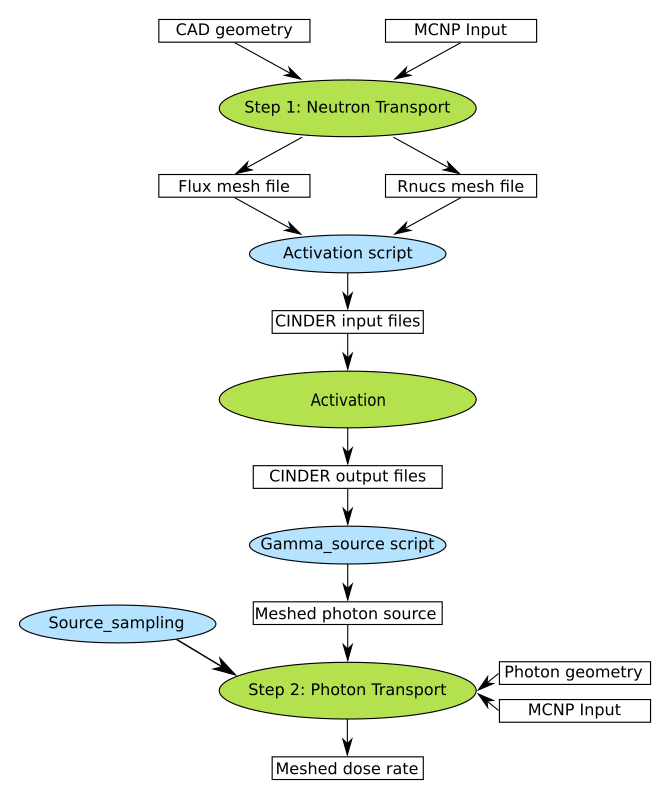
\includegraphics[scale=0.4]{../figs/rnucs_mesh.png}
\caption{Mesh RNUCS Workflow}
\label{mesh_rnucs}
\end{centering}
\end{figure}

\subsection{MCNP Patch}
The first step in the SDR  workflow is the neutron transport step.
Several changes in the MCNP source code were necessary in order to 
collect radionuclide information in a superimposed mesh.
These MCNP changes were recorded in a patch file. This file should be applied 
directly to MCNP6.1 after a DAGMC patch has been applied.
This patch DAG-MCNP6.1 will output a file with the name $r\_mesh$ which stores 
radionuclide information per voxel.
\subsubsection{Data Structure}
One key difference between the cell based rnucs R2S workflow and the mesh based
rnucs R2S workflow is the size of the array in which the data is stored.
The radionuclide production data for a cell is saved in a 1D array with
size $3*mnad$, where $mnad$ is the number of all possible nuclides
that can be created.
The nuclides that can be created in an spallation reaction
depend on the target nuclei. If the target nuclei has a mass
number A, then any nuclei with mass number A down to 1 can be
produced. In the rnucs patch this number comes from an isotope table
given as part of the input data. 

The radionuclide destruction data for a cell is also saved in a 1D array
with size $3*mndd$, where $mndd$ is the number of nuclides that make up
the material in the cell. 

The radionuclide production data for a mesh is saved in a 4D array
with size $(nxb, nyb,nzb, 3*mnad)$, where $nxb, nyb, nzb$ are the
number of bins in the $x$, $y$, and $z$ respectively. $mnad$ is the
number of all possible nuclides that can be created. 

\subsection{Activation Script}
A python script was created to collect mesh rnucs information from the $r\_mesh$
file, flux information from a meshtal file, and material information from a 
material laden CAD geometry. This collected information is then written out 
in the correct format and in the right files that can be read by the activation 
software CINDER90. 

The original perl activation script is used to read a keyword $mesh$ and call the 
python script mentioned above, write an input file for each region/voxel and run 
the CINDER90 and TABCODE software. 

\newpage
